\documentclass[class=NCU_thesis, crop=false]{standalone}
\begin{document}

\chapter{研究方法}
\section{硬體設計流程}
\subsection{模型設計軟體:Autodesk Fusion 360}
Autodesk Fusion 360是一款集合了電腦輔助設計(Computer-Aided Design, CAD)、電腦輔助製造(Computer-Aided Manufacturing, CAM)、電腦輔助工程(Computer-Aided Engineering, CAE)及印刷電路板設計(Printed Circuit Board, PCB)的多功能設計軟體。由於結合了眾多工具,所以在產品設計、工程設計、機械設計和製造等眾多領域都累積了一定規模的使用者,也成為許多設計師、工程師和製造專業人士的首選工具。

\begin{itemize}
    \item 3D建模:提供精準的參數化建模,方便使用者精準的設計每一個零件的細節。
    \item 裝配設計:模擬多個零件組合後的裝配設計,能確認組合後的零件是否能正常運作。
    \item 渲染與設計圖生成:內建強大的渲染引擎,可以生成高質量的圖像和客製化設計圖,以便更好的展示設計成果。
    \item 模型庫:官方與使用者社群建立的廣大模型庫,能找到市面上多數的電路板、馬達與零件模型,方便使用者將這些零件一起納入設計圖。
    \item 雲端協作:Autodesk擁有自己的雲端平台,團隊成員可以實時共享和協作設計,方便遠端工作和版本控制。
\end{itemize}

\begin{figure}[htbp]
    \centering
    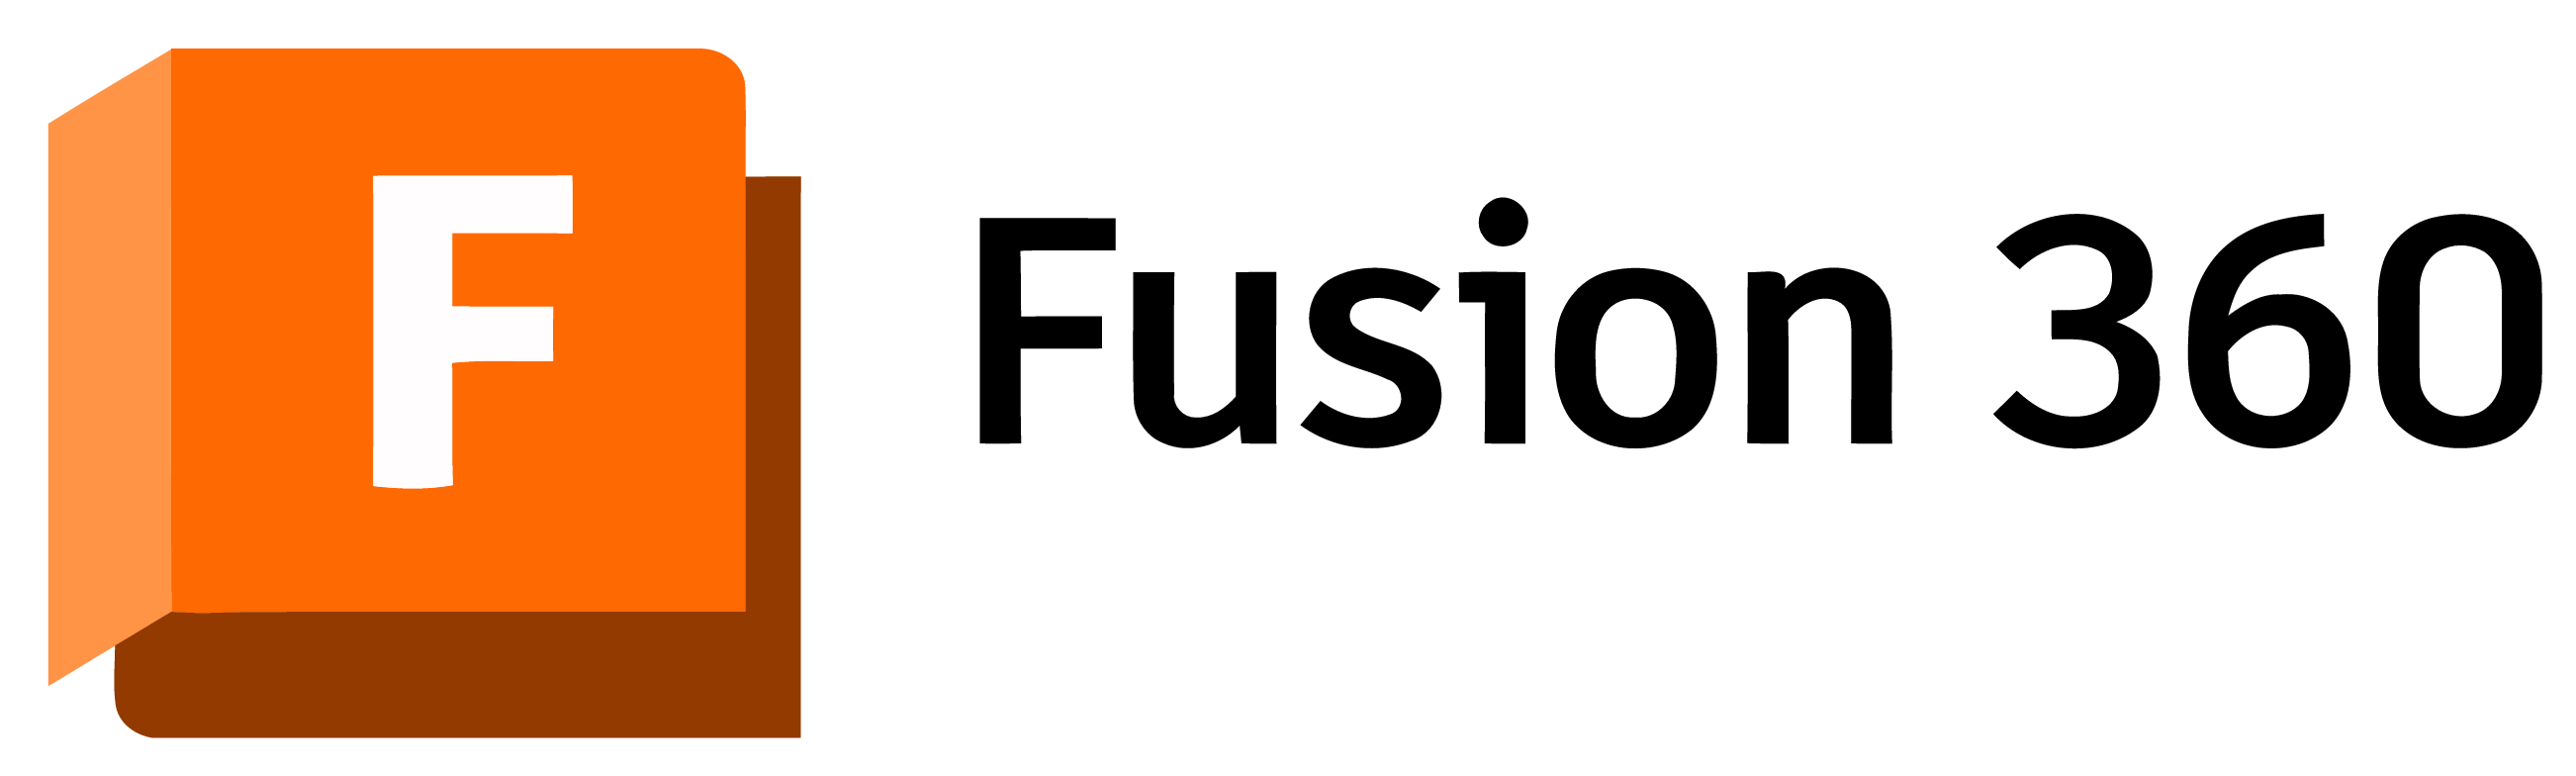
\includegraphics[width=0.75\textwidth]{figures/autodesk-fusion-360-seeklogo.png}
\caption{Autodesk Fusion 360 Logo~\cite{autodesk_echo_dot}}
\end{figure}

\subsection{檔案輸出格式:STL(Stereolithography)}
STL(Stereolithography)是一種常用的3D模型文件格式,特別是在3D列印領域中廣泛應用。STL格式最早由3D Systems公司在1987年為其立體光刻(SLA)3D列印技術開發,但隨後成為各類3D列印技術的標準文件格式。STL文件描述了3D物體的表面幾何形狀,不包含任何顏色、材質或其他屬性。以下為使用STL格式用於3D列印的優勢:

\begin{itemize}
    \item 簡單性:STL格式結構簡單,易於生成和處理。
    \item 廣泛性:幾乎所有的3D建模和3D列印軟體都支援STL檔案格式。
    \item 精度彈性:可以通過調整三角形數量來控制模型的精度和細節,適應不同的列印需求。
    \item 輕量:STL格式僅描述幾何形狀,不包含顏色、材質或其他屬性資訊,正好符合3D列印只需幾何形狀的需求。
\end{itemize}

\begin{figure}[htbp]
    \centering
    
\includegraphics[width=0.6\textwidth]{figures/3D_Systems_Logo.png}
\caption{3D Systems Logo~\cite{3dsystems_echo_dot}}
\end{figure}

\subsection{3D列印機:Creality K1 MAX}
本實驗選擇使用的3D列印機為Creality K1 MAX,以下為該機型的主要特點:
\begin{itemize}
    \item 大尺寸打印:使用CoreXY運動結構,高達300x300x300mm的列印面積,能夠滿足大型模型的列印需求。
    \item 解析度:具有極高的打印解析度,可以實現細膩的表面細節和精確的尺寸控制。
    \item 高速列印:配備了高效的運動系統和強大的驅動機構,最高能達到600mm/s的高速列印、20000mm/s²的加速度與32mm³/s 的超大流量,能夠顯著縮短列印時間。
    \item 耗材多樣性:支援多種列印耗材,包括PLA、ABS、TPU等,為使用者提供了更多創作自由度。
\end{itemize}

\begin{figure}[htbp]
    \centering
    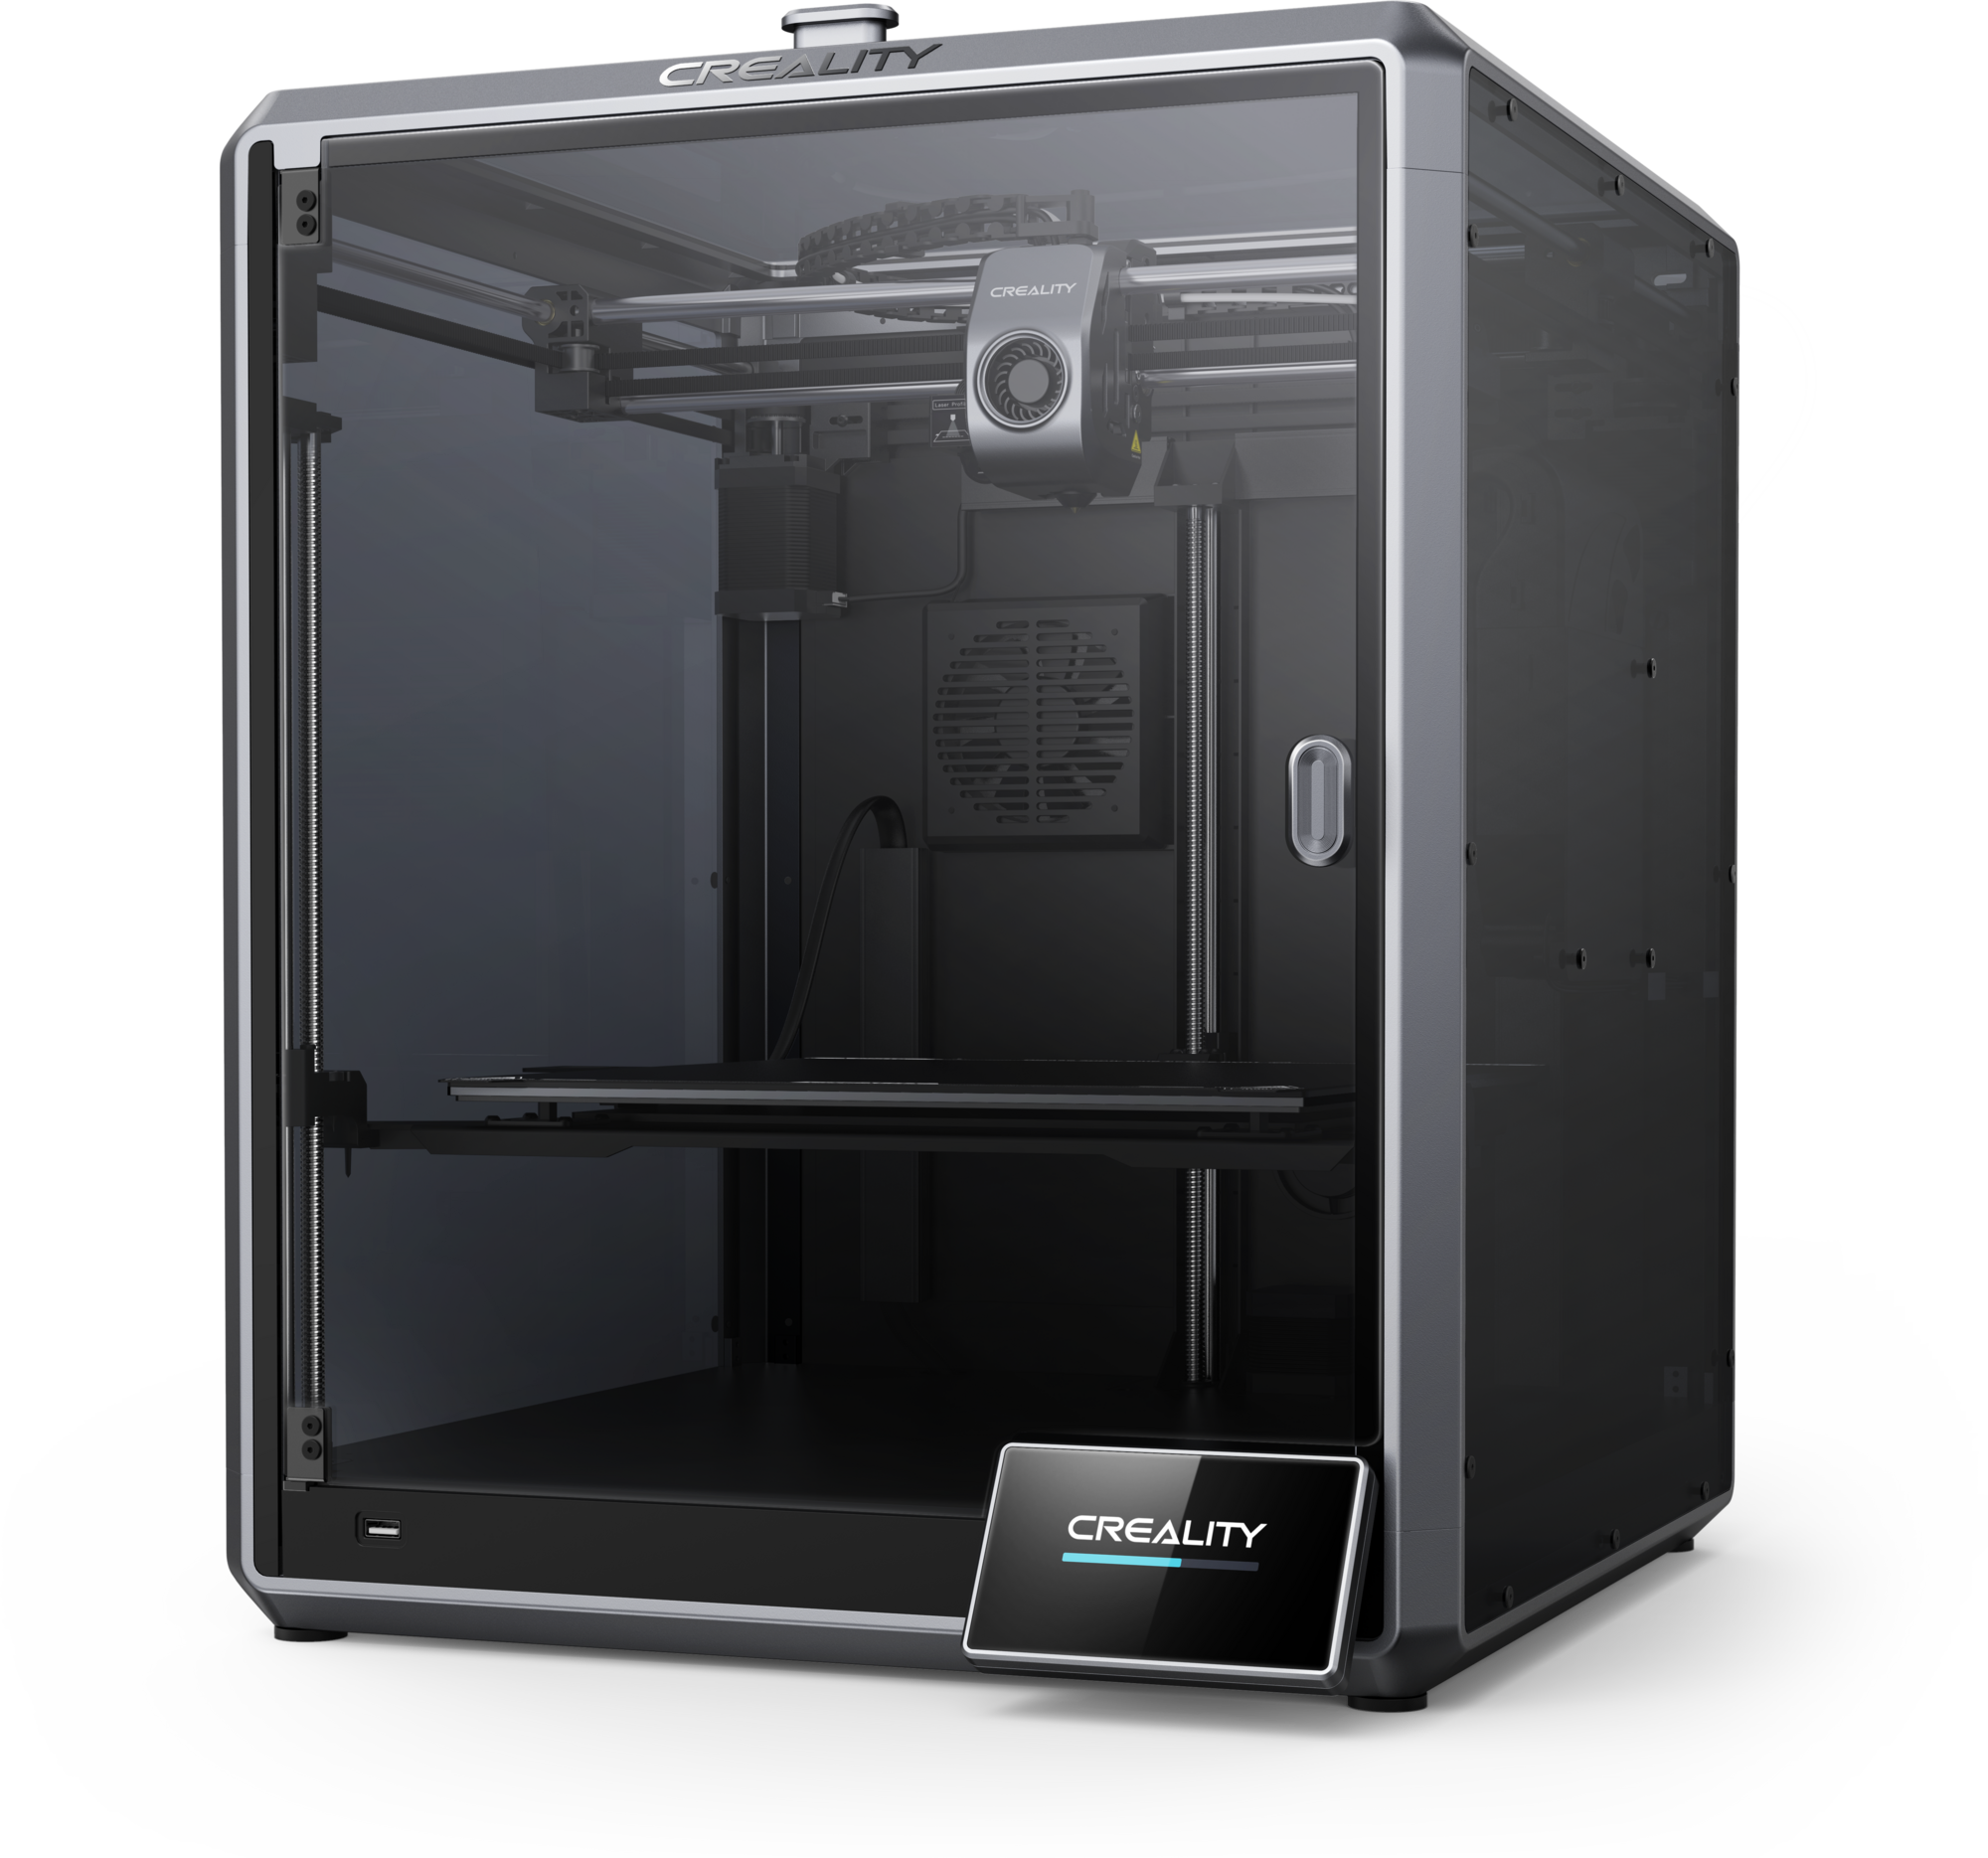
\includegraphics[width=0.5\textwidth]{figures/creality-k1-max.png}
\caption{Creality K1 MAX~\cite{creality_echo_dot}}
\end{figure}

\subsection{馬達與開發版介紹}
以下為本論文使用到的零件簡介:

\begin{enumerate}
\item SG90~\cite{sg90_servo_motor},是一款微型伺服馬達,由於扭矩較小,所以本實驗將其用於機械臂後段(操作點)。其特點包括:
\begin{itemize}
    \item 重量:小巧輕便,重量僅為9克。
    \item 操作電壓:4.8V至6.0V。
    \item 扭矩:在4.8V時可達1.8kg/cm。
    \item 控制方式:使用PWM信號來控制轉角,通常範圍為0°至180°。
\end{itemize}

\item MG90S~\cite{mg90s_servo_motor},是一款金屬齒輪伺服馬達,由於扭矩適中,所以本實驗將其用於機械臂前中段。其特點包括:
\begin{itemize}
    \item 重量:重量約為14g,稍大於SG90,但仍屬於微型伺服馬達。
    \item 操作電壓:4.8V至6.0V。
    \item 扭矩:在4.8V時可達2.2kg/cm。
    \item 控制方式:使用PWM信號來控制轉角,通常範圍為0°至180°。
\end{itemize}

\item MG996R~\cite{mg996r_servo_motor},是一款高扭矩伺服馬達,由於扭矩較大,所以本實驗將其用於機械臂前段。其特點包括:
\begin{itemize}
    \item 尺寸:重量約為55g,適用於中型或大型專案。
    \item 操作電壓:4.8V至7.2V。
    \item 扭矩:在6.0V時可達9.4kg/cm。
    \item 控制方式:使用PWM信號來控制轉角,通常範圍為0°至180°。
\end{itemize}

\item Raspberry Pi 4~\cite{raspberry_pi_4},是一款高性能的嵌入式裝置。其特點包括:
\begin{itemize}
    \item 處理器:四核ARM Cortex-A72,1.5GHz。
    \item 內存:有2GB、4GB和8GB可選,本實驗採用8GB內存。
    \item 輸入/輸出:支援USB 3.0、HDMI、GPIO、以太網等連接方式,同時也支援wifi藍芽等無線連接方式
    \item 作業系統:本實驗採用Raspberry Pi OS(基於Debian)。
\end{itemize}

\item ESP32-S3-Devkit~\cite{esp32_s3_devkit},是一款高性能、低功耗的微控制器,適合用於物聯網應用。其特點包括:
\begin{itemize}
    \item 處理器:雙核Xtensa LX7,最高240MHz。
    \item 內存:512KB SRAM,支持外部RAM擴展。
    \item 輸入/輸出:支援microUSB連接方式,同時也支援Wi-Fi和藍芽等無線連接方式。
    \item 作業系統:本實驗採用circuit python。
\end{itemize}

\item ESP32 Doit-Devkit~\cite{esp32_doit_devkit},是一個常見的ESP32開發板,設計簡單且功能強大。其特點包括:
\begin{itemize}
    \item 處理器:雙核Xtensa LX6,最高240MHz。
    \item 內存:520KB SRAM。
    \item 支援microUSB連接方式,同時也支援Wi-Fi和藍芽等無線連接方式。
    \item 作業系統:本實驗採用circuit python。
\end{itemize}

\item L298N~\cite{l298n_motor_driver},直流馬達驅動模組,常用於控制雙馬達系統,本實驗將此裝置用於控制車輪。其特點包括:
\begin{itemize}
    \item 電壓範圍:可操作電壓範圍為5V至35V。
    \item 電流:每通道峰值電流可達2A。
    \item 控制:使用PWM訊號控制馬達速度和方向。
\end{itemize}

\item PCA9685~\cite{pca9685_pwm_driver},是一款16通道PWM驅動模組,通常用於控制伺服馬達和LED燈,本實驗將此裝置用於控制機械臂馬達。其特點包括:
\begin{itemize}
    \item PWM頻率:可調頻率範圍為24Hz至1526Hz。
    \item 接口:使用I2C介面進行訊號傳輸。
    \item 控制:使用PWM訊號控制馬達速度和方向,適合需要一次性控制大量馬達的專案。
\end{itemize}
\end{enumerate}
\begin{figure}[!hbt]
    \centering
    \subcaptionbox
        {SG90~\cite{sg90_servo_motor}
        \label{fig:fig-dataset-contrast-after-adjustment}}
        {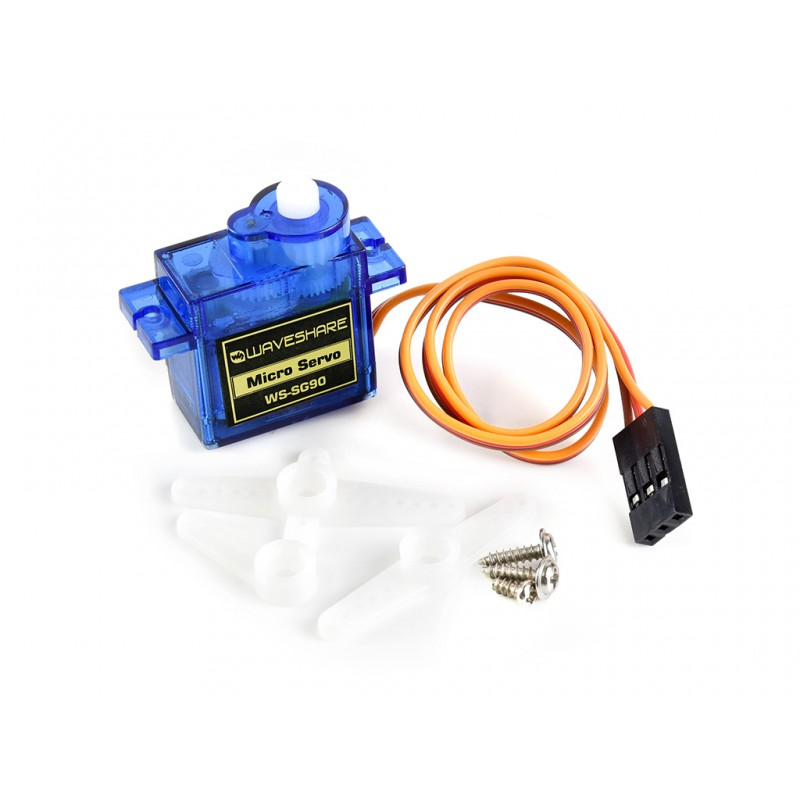
\includegraphics[width=0.25\linewidth]{figures/SG90.jpg}}
    ~    
    \subcaptionbox
        {MG90S~\cite{mg90s_servo_motor}
        \label{fig:fig-dataset-contrast-after-adjustment}}
        {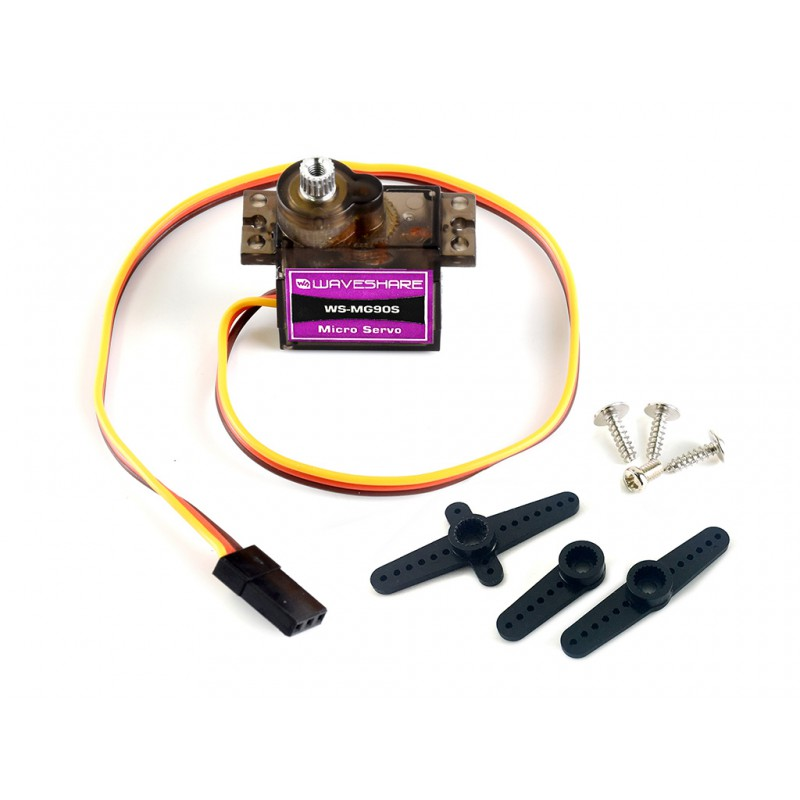
\includegraphics[width=0.25\linewidth]{figures/MG90S.jpg}}
    ~    
    \subcaptionbox
        {MG996R~\cite{mg996r_servo_motor}
        \label{fig:fig-dataset-contrast-after-adjustment}}
        {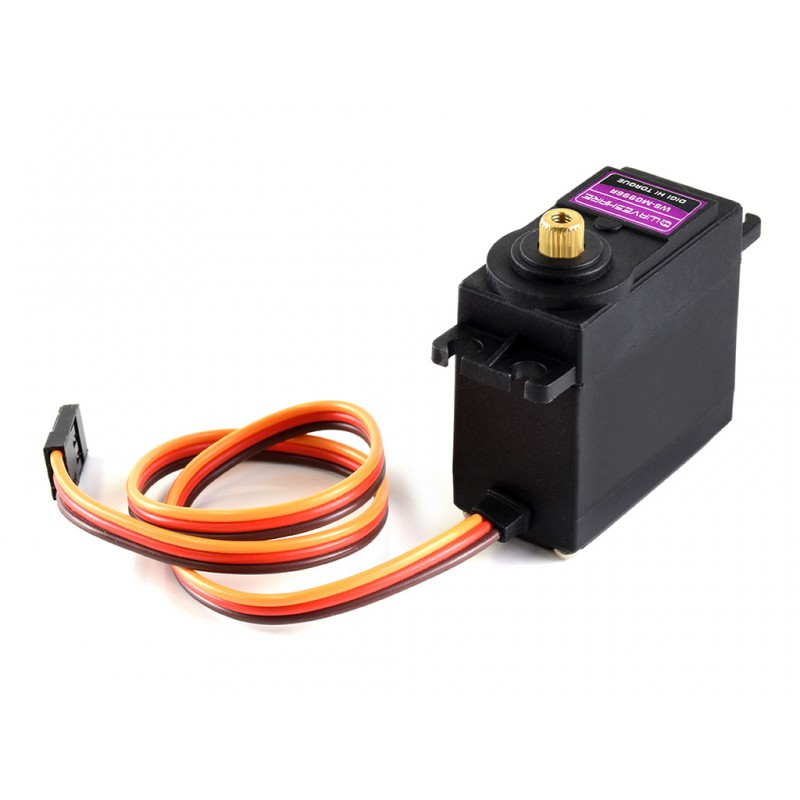
\includegraphics[width=0.25\linewidth]{figures/MG996R.jpg}}
    ~   
    \subcaptionbox
        {Raspberry Pi 4~\cite{raspberry_pi_4}
        \label{fig:fig-dataset-contrast-after-adjustment}}
        {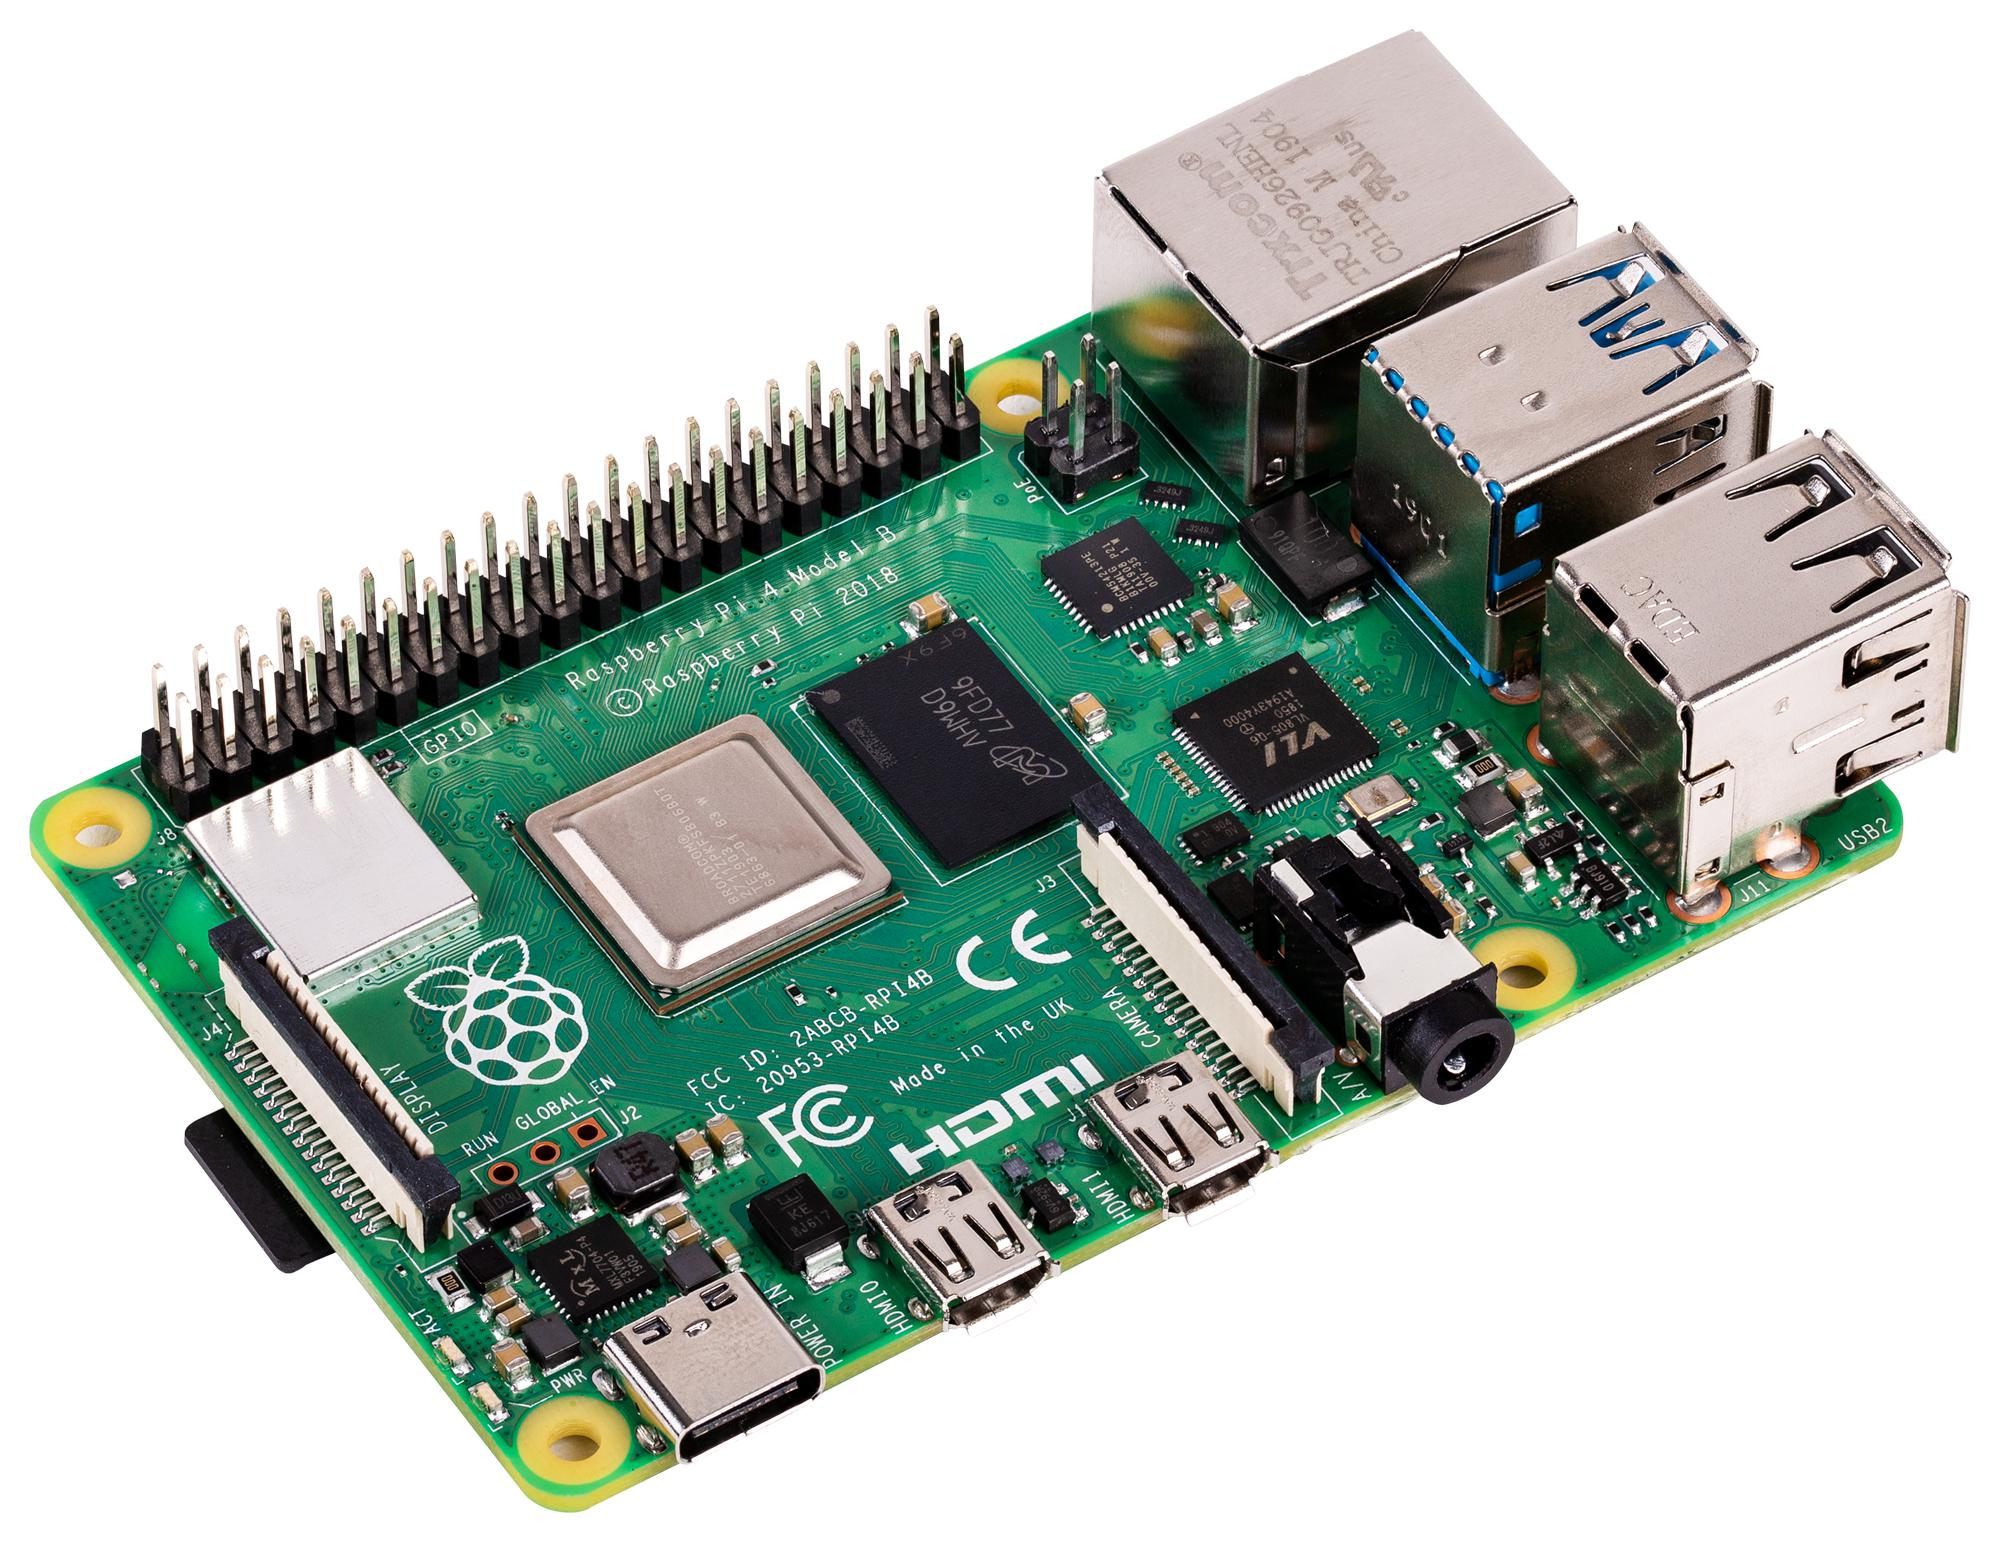
\includegraphics[width=0.25\linewidth]{figures/Rasberry pi 4.jpg}}
    ~    
    \subcaptionbox
        {ESP32-S3-Devkit~\cite{esp32_s3_devkit}
        \label{fig:fig-dataset-contrast-after-adjustment}}
        {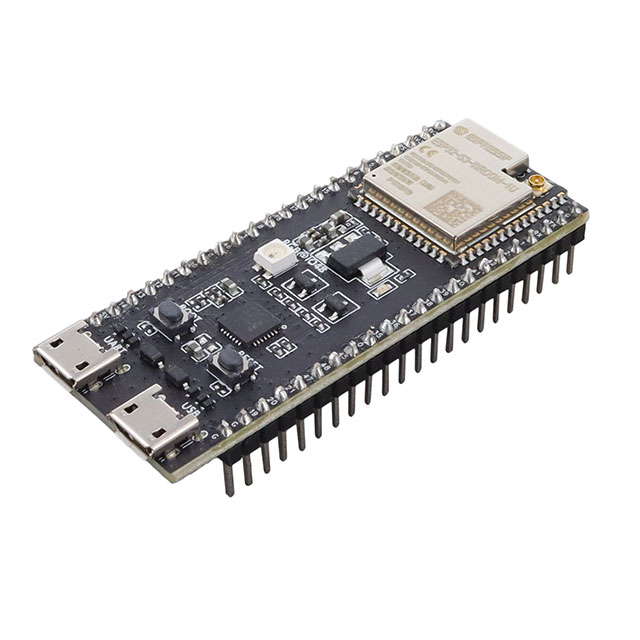
\includegraphics[width=0.25\linewidth]{figures/ESP32-S3.jpg}}
    ~    
    \subcaptionbox
        {ESP32 Doit-Devkit~\cite{esp32_doit_devkit}
        \label{fig:fig-dataset-contrast-after-adjustment}}
        {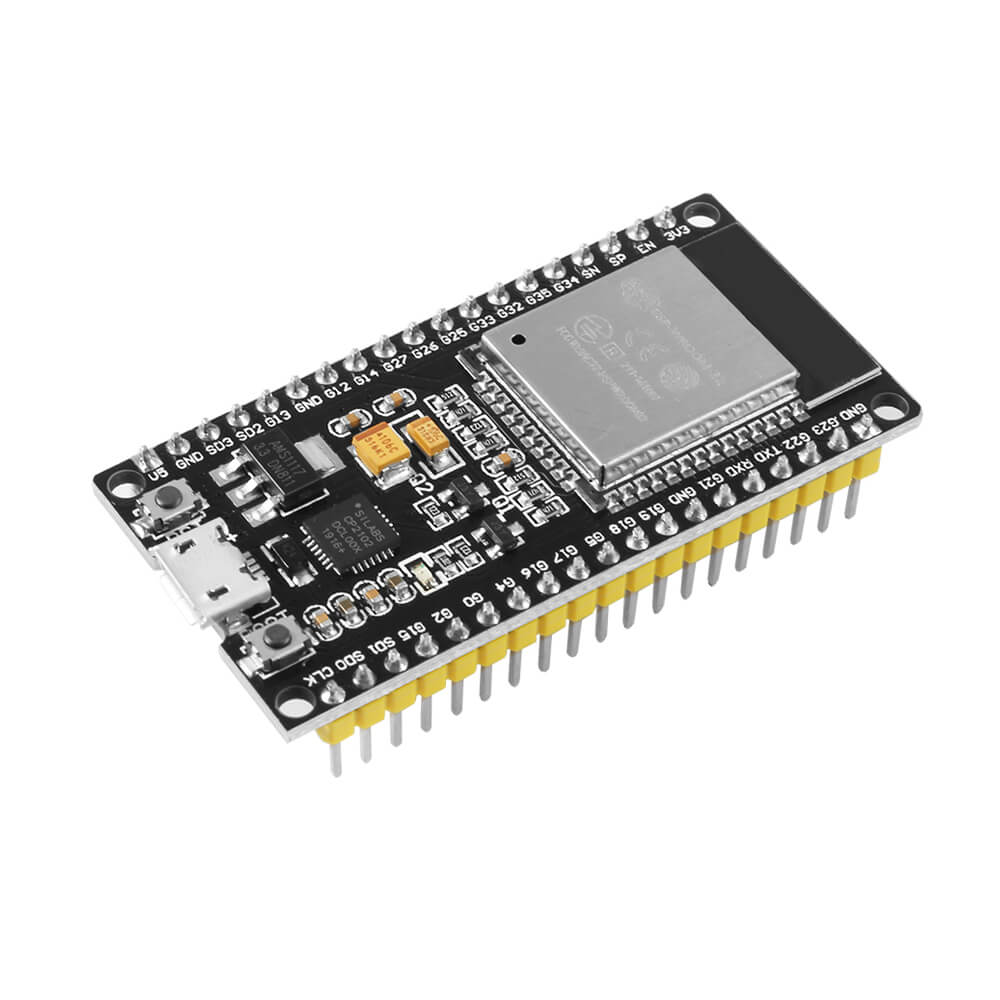
\includegraphics[width=0.25\linewidth]{figures/ESP32-DOIT.jpg}}
    ~  
    \subcaptionbox
        {L298N~\cite{l298n_motor_driver}
        \label{fig:fig-dataset-contrast-after-adjustment}}
        {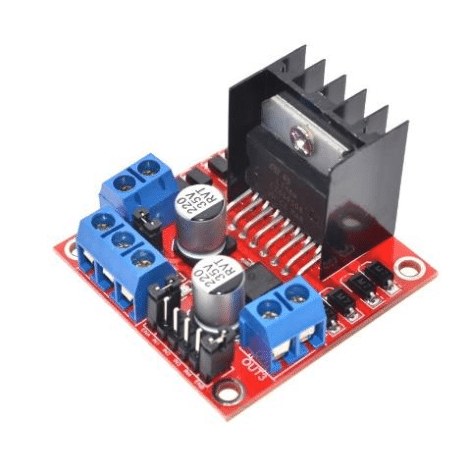
\includegraphics[width=0.25\linewidth]{figures/L298N.png}}
    ~    
    \subcaptionbox
        {PCA9685~\cite{pca9685_pwm_driver}
        \label{fig:fig-dataset-contrast-after-adjustment}}
        {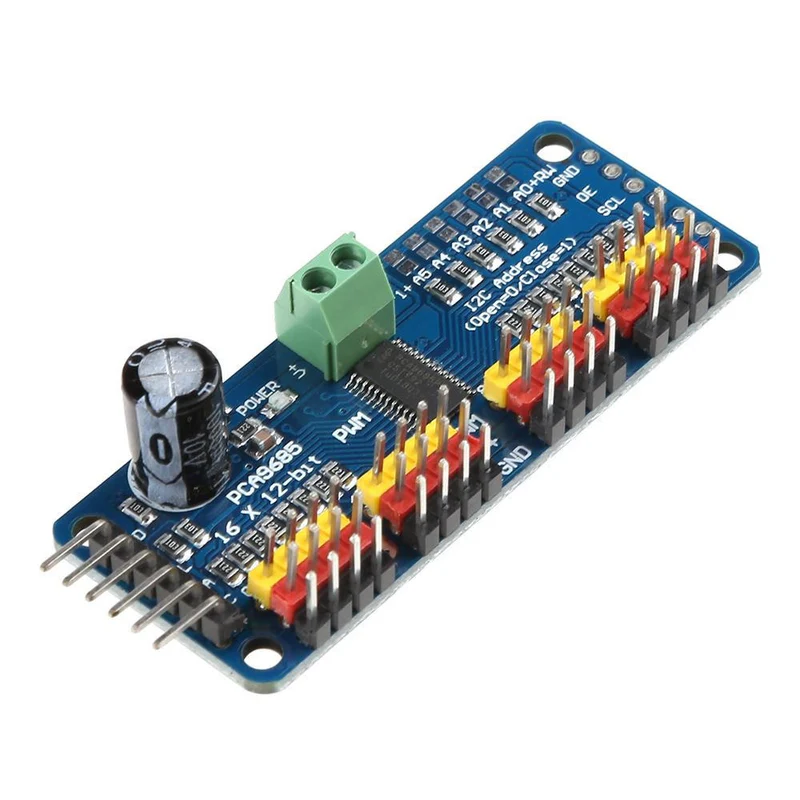
\includegraphics[width=0.25\linewidth]{figures/PCA9685.png}}
\caption{開發板與馬達縮圖}
\end{figure}

\section{運動學開發}

\subsection{運動模擬環境}
本專案使用Python語言開發了一個簡易的機械臂模擬環境。這個模擬環境的基本原理,是將機械臂定義為一個擁有多個可調整參數的獨立物件,其中包括力臂長度、扭轉角、節點偏移、節點角度、目標頂點、和目前頂點等。這些參數可以由使用者根據需求進行調整,從而在虛擬空間中生成機械臂的模型。該模擬環境提供了一個直觀且靈活的介面,使得使用者能夠方便地設計和測試機械臂的運動行為。

\begin{listing}
    \begin{minted}[frame=single,
                   framesep=3mm,
                   linenos=true,
                   xleftmargin=21pt,
                   tabsize=4]{python}

        class ArmEnv_3D:
            def __init__(self, lList, vision=True):
                self.Link_length = lList
                self.Link_offset=[0]*len(lList)
                self.Twist_angle=[0]*len(lList)
                self.Joint_angle = [0]*len(lList)
                self.Target_point=[0, 0, 0]
                self.Current_point=[0, 0, sum(lList)]

            def Forward_kinematics(self, joint_angles):...
            
            def Geometric_solution(self):...

            def Gradient_policy(self,times=100, points=10, speed=5):...

            def initPicture(self):...

            def updatePicture(self):...

    \end{minted}
\caption{運動模擬環境程式架構} 
\end{listing}

\subsection{順向運動學}
在順向運動學部分,本專案採用了Denavit-Hartenberg方法作為主要的計算方式。這種方法能夠系統地描述和計算機械臂的運動行為。模擬環境中的相關函式可以直接被呼叫,利用即時的機械臂參數來計算操作點的空間座標。計算結果會即時顯示在模擬空間中。

\subsection{逆向運動學}
在逆向運動學方面,本專案結合了幾何求解(Geometric solution approach)方法和策略梯度(Policy-Gradient solution approach)方法來進行計算。幾何求解方法主要用於計算運動模式較為簡單的機械臂,而策略梯度方法則適用於運動較為複雜的機械臂。這些計算函式同樣可以在模擬環境中直接被呼叫。根據輸入的目標操作點位置,系統會計算出對應的扭轉角,並將結果顯示在模擬空間中。

\section{大型語言模型開發}
\subsection{OpenAI與GPT模型}
本實驗使用的大型語言模型為OpenAI所推出的GPT(Generative Pre-trained Transformer)模型,GPT模型是一種基於變換器(Transformer)架構的生成式預訓練模型,用於應對自然語言處理相關的任務。自推出以來,此模型已經經歷了多次迭代,從最初的GPT-1到最新的GPT-4o,每一代都在參數量、性能與應用靈活度上取得了顯著的進步。這些模型通過在大規模文本數據上進行預訓練,能夠生成高品質文字、圖片等資訊。

\subsection{模型使用流程}
呼叫OpenAI chat-GPT API的流程,簡單可以分為以下幾個步驟:
\begin{enumerate}
    \item 註冊與獲取密鑰:在OpenAI的官方網站上註冊一個帳號,並建立一個API密鑰。
    \item 安裝必要的函式庫:本實驗使用python作為開發語言,所以需要在開發環境中安裝對應版本的函式庫。
    \item 在程式中設置密鑰:在程式碼中設定建立好的密鑰,以供官方伺服器驗證。
    \item 發送請求與處理回應:接下來即可向伺服器發送請求,並處理文本回應。
\end{enumerate}
\newpage
在對GPT模型下達指令時,需要將預計上傳的文字資訊封裝成特定格式,以下為簡易範例:\\

\begin{listing}[h]
    \begin{minted}[frame=single,
                   framesep=3mm,
                   linenos=true,
                   xleftmargin=21pt,
                   tabsize=4]{js}
        {
          "model": "model_type",
          "prompt": "介紹一下OpenAI和GPT模型。",
          "max_tokens": 100,
          "temperature": 0.7,
          "top_p": 1.0,
          "n": 1,
          "stop": null
        }
    \end{minted}
\caption{JSON請求範例} 
\end{listing}

\begin{listing}[h]
    \begin{minted}[frame=single,
                   framesep=3mm,
                   linenos=true,
                   xleftmargin=21pt,
                   tabsize=4]{sh}

        curl https://api.openai.com/v1/completions \
          -H "Content-Type: application/json" \
          -H "Authorization: Bearer API密鑰" \
          -d '{
            "model": "model_type",
            "prompt": "介紹一下OpenAI和GPT模型。",
            "max_tokens": 100,
            "temperature": 0.7,
            "top_p": 1.0,
            "n": 1,
            "stop": null
          }'
    \end{minted}
\caption{HTTP請求範例} 
\end{listing}

以下為主要參數說明:
\begin{itemize}
    \item model: 指定使用的GPT模型,例如text-davinci-004、GPT-4o、GPT-3.5等。
    \item prompt: 下達的指令。
    \item max\_tokens: 回傳文字的最大長度。
    \item temperature: 控制生成文字的隨機性。此值越高會生成更具創造性的文字,反之值越低則生成越保守的文字。
    \item top\_p: 取樣方法,決定生成文本的多樣性。
    \item n: 返回生成文章的數量。
    \item stop: 用於指定生成文字停止的條件,可設定為空值。
\end{itemize}
\newpage

\section{系統架構}
\subsection{系統架構與流程}
本實驗的系統架構與流程大致如下:
\begin{enumerate}
    \item GUI上傳使用者輸入至Server:使用者在GUI上輸入文字並上傳至伺服器。
    \item Server上傳使用者輸入至OpenAI API:伺服器將這些使用者輸入發送至OpenAI API。
    \item OpenAI API回傳模型輸出至Server:OpenAI API處理輸入並回傳模型生成的輸出至伺服器。
    \item Server將輸出傳送至指定的機器:伺服器將這些輸出數據傳送至指定的機器,進行控制。
    \item Server向GUI回傳伺服器與機器狀態:最後,伺服器將機器和自身的狀態訊息回傳至GUI,讓使用者了解系統運行情況。
\end{enumerate}
\clearpage
\begin{figure}[h]
    \centering
    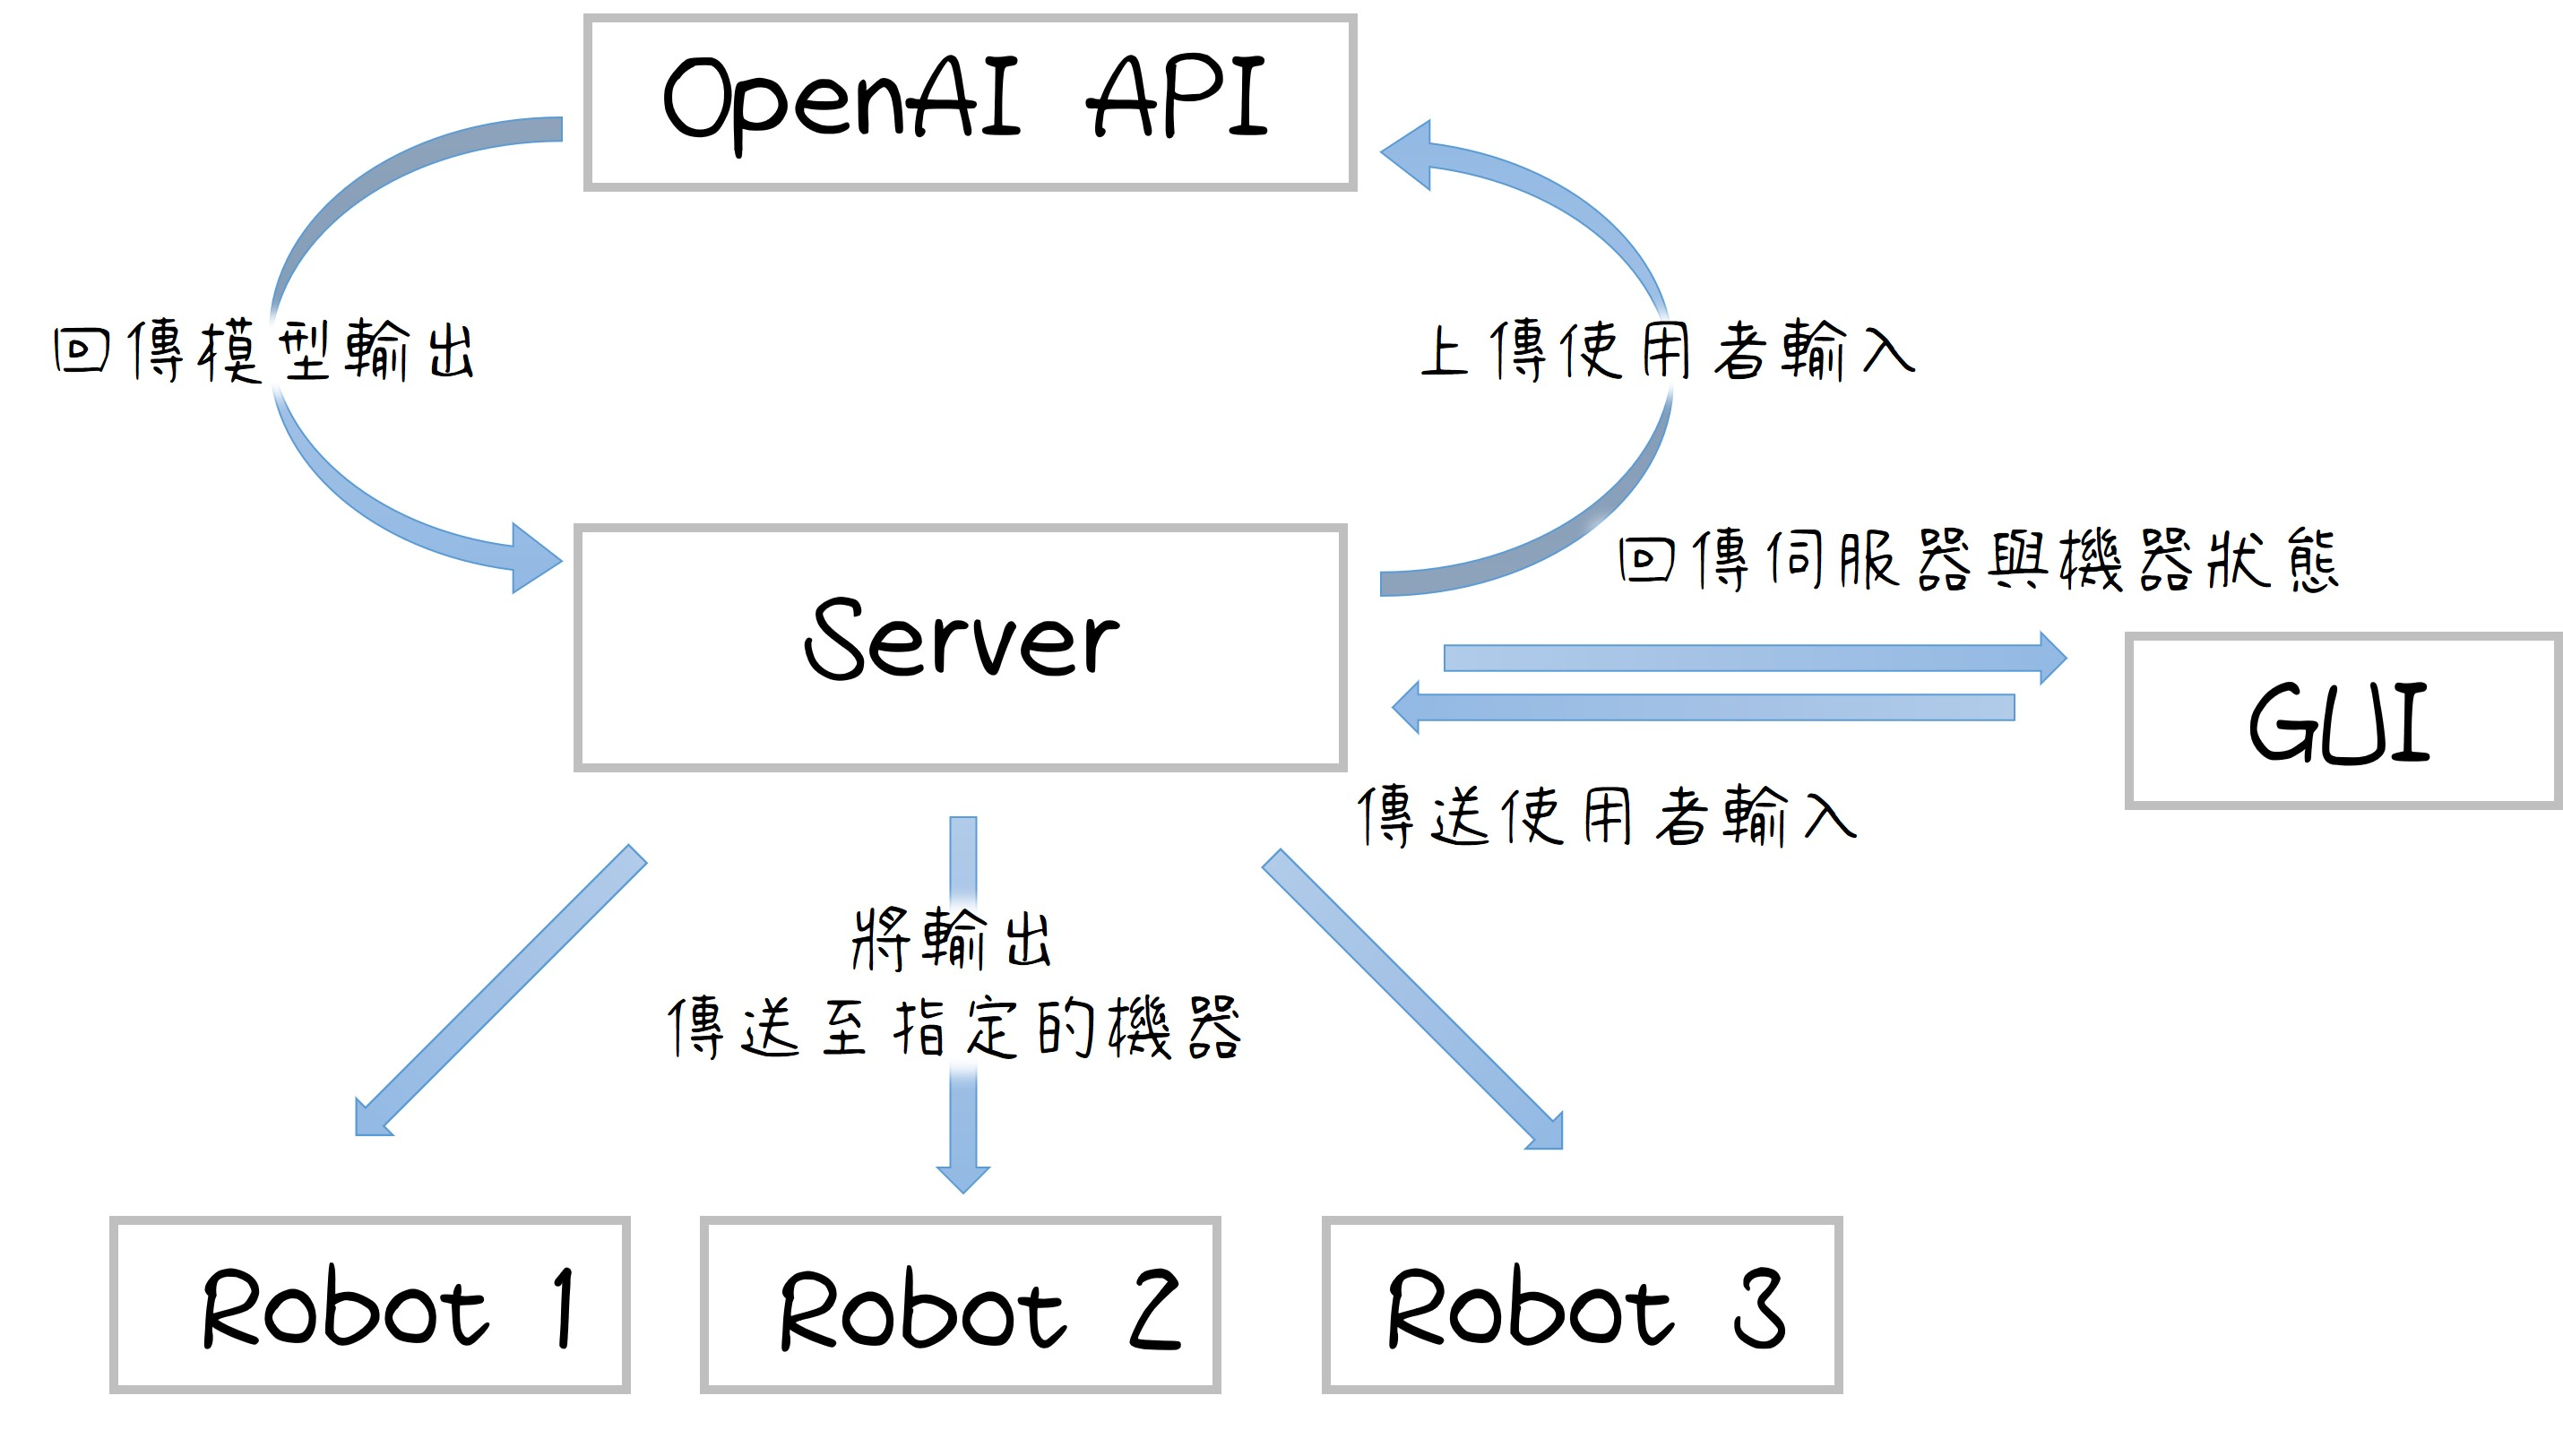
\includegraphics[width=0.6\textwidth]{figures/structure.jpg}
    \caption{系統架構圖}
\end{figure}

\begin{figure}[h]
    \centering
    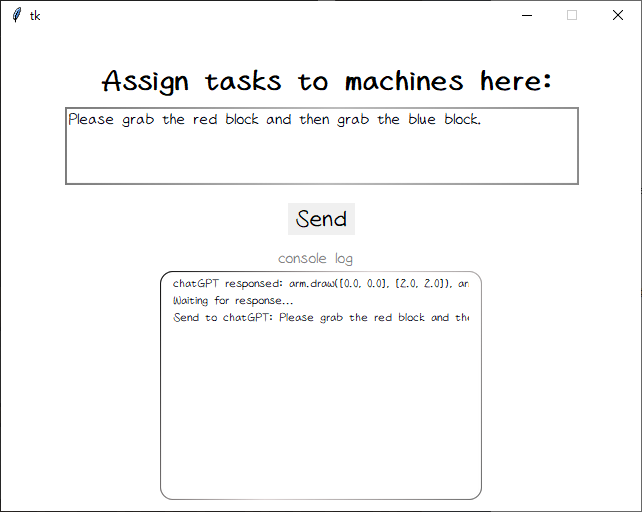
\includegraphics[width=0.6\textwidth]{figures/GUI.png}
    \caption{使用者介面縮圖}
\end{figure}



\end{document}